\section{Instalação do Octave}
\label{sec:instal}

A primeira coisa que você deve fazer é instalar o GNU Octave em seu computador.
Caso você já tenha o Octave instalado, incluindo os packages extras mencionados
abaixo, vá para a próxima seção. Caso contrário, continue lendo.

Existem instaladores do Octave para Linux, Windows e Mac. Vá até o site principal
do Octave em \url{https://www.gnu.org/software/octave/} e faça o download do
instalador apropriado (sistemas Linux geralmente não precisam fazer download
do Octave, basta instalar através do gerenciador de pacotes de sua distribuição).
Em caso de dificuldade consulte a documentação
(\url{https://wiki.octave.org/Category:Installation}) ou solicite auxílio ao
monitor da disciplina.

Após a instalação terminar inicie o Octave. Você deve ver algo parecido com
a figura~\ref{fig:octave-gui}:

\begin{figure}[!h]
  \begin{center}
    \caption{Octave 5.1.0 em um computador Linux}
    \label{fig:octave-gui}
    %\fbox{
       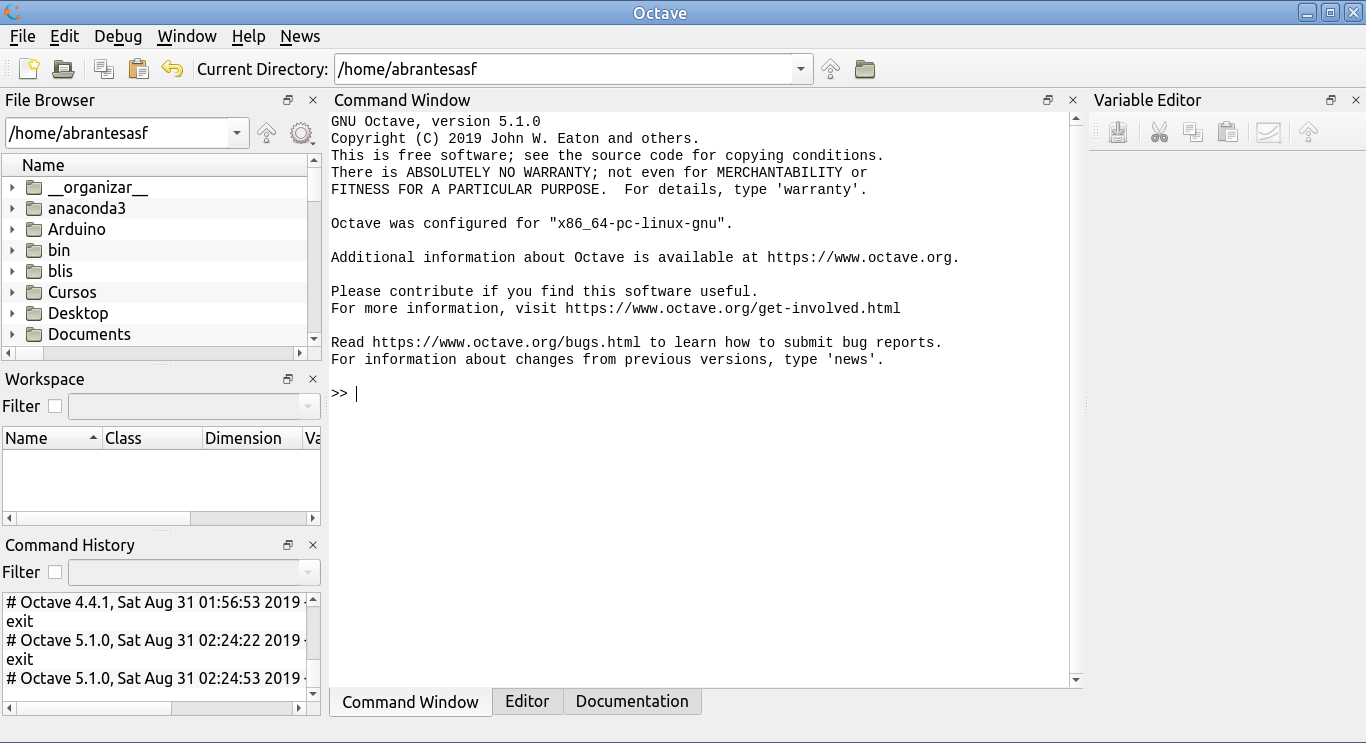
\includegraphics[scale=0.3]{imagens/octave-gui.png}
    %}
    %\footnotesize{Fonte:~\citet[][]{citação}}
  \end{center}
\end{figure}

Uma característica interessante do Octave é que ele permite que vários outros
\ingles{packages} com funcionalidades extras possam ser adicionados à instalação
base. Visite o repositório de pacotes adicionais em
\url{https://octave.sourceforge.io/packages.php} e veja quantas funcionalidades
avançadas e específicas já estão disponíveis. Nós faremos a instalação dos
seguintes pacotes adicionais:

\begin{itemize}[noitemsep]
\item symbolic
\item general
\item optim
\item data-smoothing
\item statistics
\item image
\item io
\end{itemize}

Para instalar o pacote \ingles{symbolic}, por exemplo, devemos digitar na
janela de comando do Octave o seguinte:
\begin{tcolorbox}
\begin{lstlisting}[language=bash]
pkg install -forge symbolic
\end{lstlisting}
\end{tcolorbox}

Durante a instalação dos pacotes podem aparecer avisos diversos e \ingles{warnings}
que podem ser ignorados se, no final de tudo aparecer uma mensagem semelhante
à ``For information about changes from previous versions of the symbolic package,
run 'news symbolic''', que indica que o pacote foi instalado com sucesso.

Instale todos os pacotes da lista acima (caso um pacote seja pré-requisito para
outro, o Octave emitirá um aviso e você deverá ajustar a ordem de instalação).
